Cai et al. \cite{caiMSTMultistageSpectralwise2022a} propose the Multi-stage Spectral-wise Transformer (MST),
for the task of spectral super resolution.
The idea the authors introduce, is instead of forming tokens by partitioning the spatial domain,
entire spectral-bands are being treated as tokens.
Given a feature map $X \in \mathbb R^{C \times H \times W}$, the spatial domain is flattened,
leading to the shape $C \times HW$,
each entry in the channel dimension is then treated as a token, 
yielding $(x_k)_{k=1}^{C} \in \mathcal S( \mathbb R^{HW})$.
The model architecture is depicted in figure \ref{fig:mst}.

\begin{figure}[h!]
    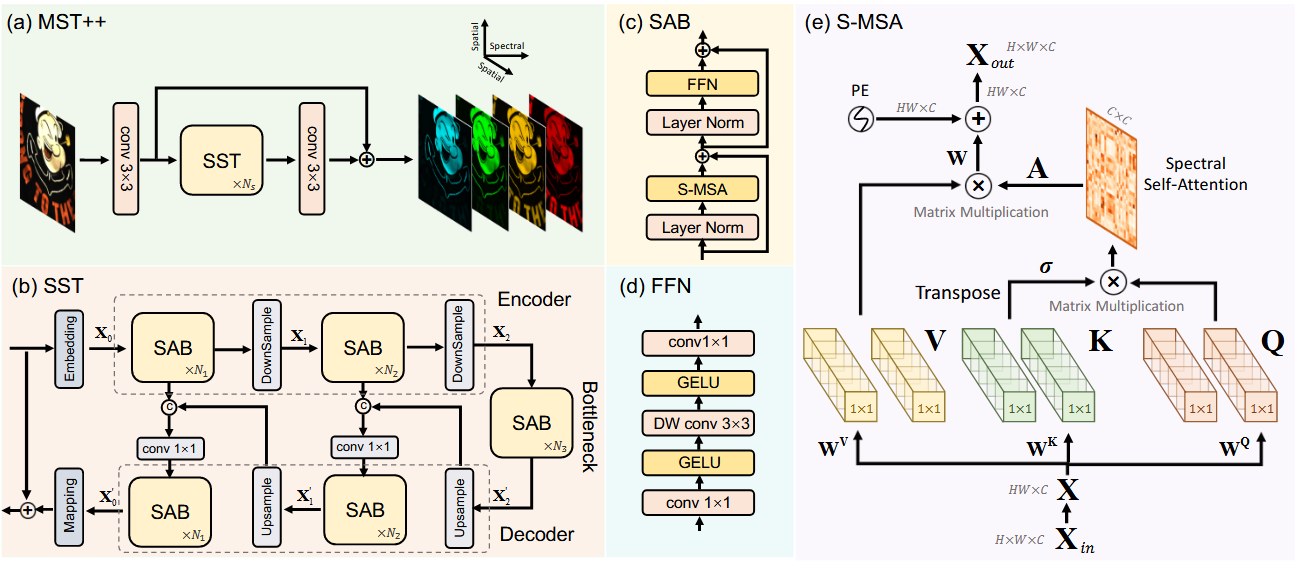
\includegraphics[width=0.9\textwidth]{models/ssr/imgs/mst.png}
    \caption{Image taken from \cite{caiMSTMultistageSpectralwise2022a}, architecture of MST model.}
    \label{fig:mst}
\end{figure}

The deep feature extraction module $H_d$ consists of $3$ cascaded SIngle-stage Spectral-wise Transformers (SSTs),
followed by a final convolutional layer

    $$ H_d = C \circ H_{SST} \circ ... \circ H_{SST} ~. $$

An SST admits a U-Net like architecture, displayed in part (b) of figure \ref{fig:mst}.

A SAB is a variation of a Transformer Block as described in definition \ref{def:transformer_block}.
Instead of standard multi-headed self-attention, spectra-wise self-attention is used.
Given an input $X \in \mathbb R^{C \times H \times W}$ tokens $(x_{k = 1})^C \in \mathcal S (\mathbb R^{HW})$ are formed,
as described in the introduction.
The tokens are embedded using matrices $Q_h, K_h, V_h \in \mathbb R^{d_h \times C}$,
for $h = 1, ..., H$, as in standard multi-headed self-attention, 
to obtain provisional queries and keys $(\hat{q}_k^{(h)})_{k=1}^{HW}, (\hat{k}_k^{(h)})_{k=1}^{HW}$ 
as well as values $(\hat{v}_k^{(h)})_{k=1}^{HW}$, that is

    $$ \hat{q}_k^{(h)} = Q_h x_k, \hat{k}_k^{(h)} = K_h x_k \text{ and } \hat{v}_k^{(h)} = V_h x_k ~. $$

In contrary to standard self-attention the tokens are then transposed in some sense, 
to obtain final queries and keys $(q_k^{(h)})_{k=1}^{C}, (k_k^{(h)})_{k=1}^{C}$
given by

    $$ q_k^{(h)}(i) = \hat{q}_i^{(h)}(k) \text{ and } k_k^{(h)}(i) = \hat{k}_i^{(h)}(k) ~, $$

for $i = 1, ..., HW$ and $k = 1, ..., C$.
To the computation of attention scores an optimizable scalar $\sigma_j \in \mathbb R$ is introduced,
for keeping the magnitude of the dot product in check,
instead of a fixed factor,
as spectral density varies with respect to the wavelength

    $$ A_{ij}^{(h)} = \frac{\text{exp} \left( \sigma_j {k_{i}^{(h)}}^\top q_{j}^{(h)} \right)}{\sum_{k = 1}^n \text{exp} \left( \sigma_j {k_{k}^{(h)}}^\top q_{j}^{(h)} \right)} $$

for $i, j = 1, ..., d_h$.
Finally 

    $$y_j^{(h)} = \sum_{i=1}^{C} A_{ij}^{(h)} v_j^{(h)} ~, $$

Using a optimizable matrix $W \in \mathbb R^{C \times C}$, 
the heads are merged back together 

    $$y_k = W [y_k^{(1)}, ..., y_k^{(H)}] ~, $$

for $k = 1, ..., HW$.

\begin{figure}[h!]
    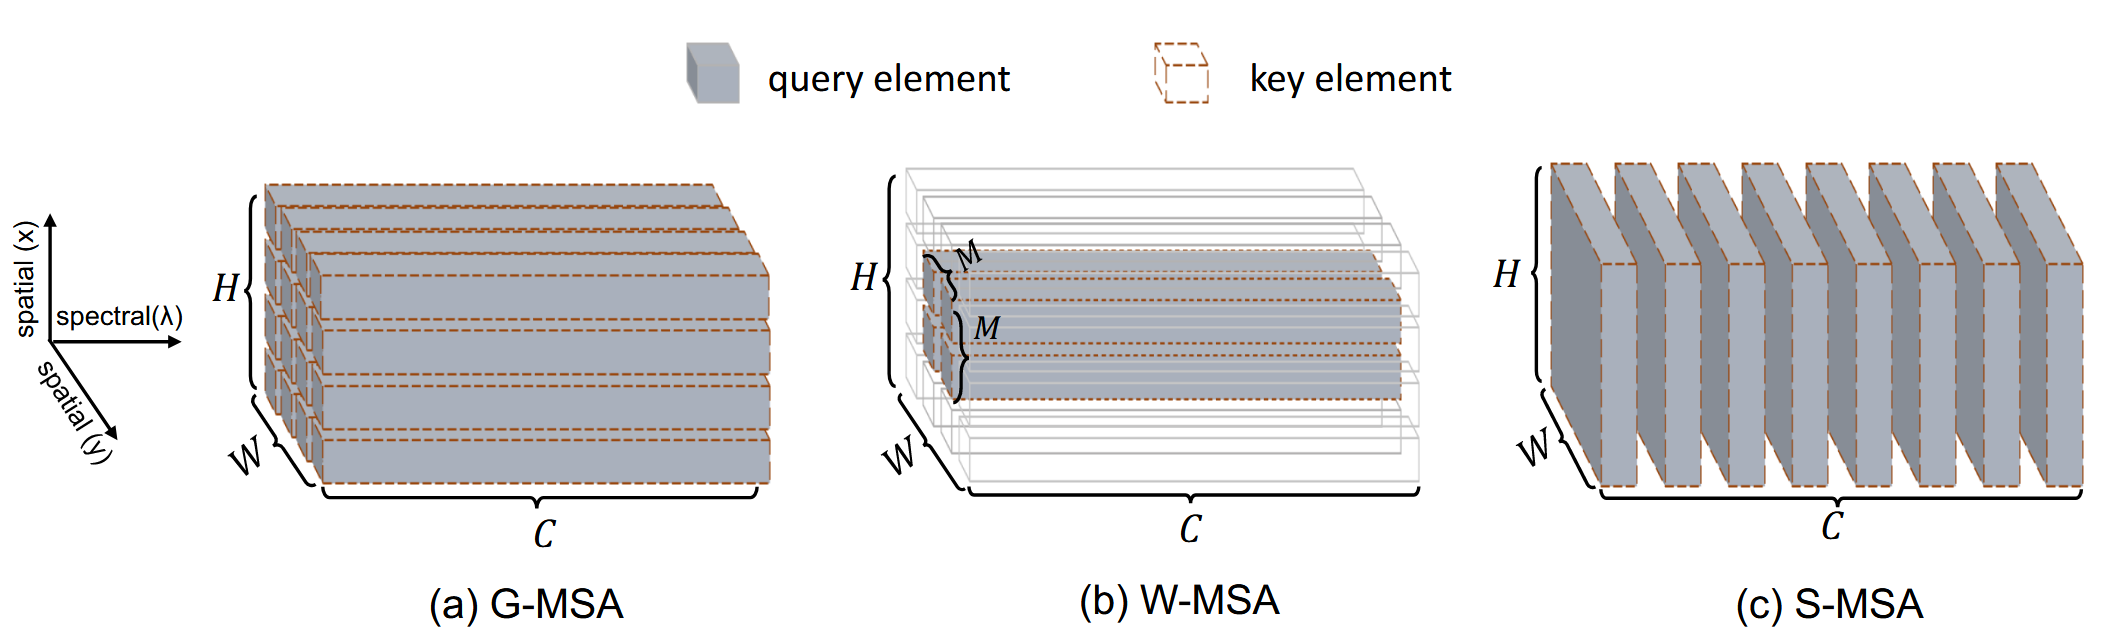
\includegraphics[width=0.9\textwidth]{models/ssr/imgs/smsa.png}
    \caption{Image taken from \cite{caiMSTMultistageSpectralwise2022a}, Spectral Multi-headed Self-Attention.}
    \label{fig:smsa}
\end{figure}